\documentclass[11pt]{article}
\usepackage{graphicx}
\usepackage{float}
\usepackage{amsmath}
\usepackage{amssymb}
\usepackage{dirtytalk} % For \say{}
\usepackage{hyperref}
\hypersetup{
    colorlinks=true,
    }

\setlength{\textwidth}{6.5in}
\setlength{\headheight}{0in}
\setlength{\textheight}{8.0in}
\setlength{\hoffset}{0in}
\setlength{\voffset}{0in}
\setlength{\oddsidemargin}{0in}
\setlength{\evensidemargin}{0in}

\def\dbar{{\mathchar'26\mkern-12mu d}}

\title{2D Ising Models Draft 2}
  
\author{Salar Ghaderi, Xinyu Liu, and Tongzhou Wang}
\date{November 19, 2024}

\begin{document}

\maketitle

\abstract{We perform a Markov chain Monte Carlo simulation of the energy and magnetization of a heating two-dimensional square lattice Ising model initially at absolute zero with all spins aligned. We also perform the simulation for a cooling system initially above the critical temperature with random spin orientations. For this second draft, we report and discuss each of our results separately, which we will work on to integrate soon.}

\section{Introduction}

\subsection{The Ising Model}
The Ising model is a theoretical model of ferromagnetism proposed by Ernst Ising in 1925 \cite{ising1925contribution, kramers1941statistics}. In the two-dimensional square lattice Ising model, a magnetic material is modeled by a two-dimensional square lattice with magnetic dipoles on the lattice sites. The magnetic dipoles are assumed to be capable of pointing in only two directions, up or down, characterized by $s = \pm 1$. It is further assumed that a magnetic dipole interacts only with its four nearest neighbors (for dipoles on the edges, periodic boundary conditions are assumed). Thus, the total energy of the system is given by
\begin{equation}
    E = -J \sum_{\langle ij \rangle} s_i s_j - H \sum_{i} s_i,
\end{equation}
where $J$ is a positive interaction constant and $H$ accounts for an external magnetic field. The notation $\langle ij \rangle$ indicates a sum over pairs $s_i$, $s_j$ that are adjacent on the lattice.

For a system of $N \times N$ dipoles, the magnetization (magnetic dipole moment density) can be characterized by
\begin{equation}
    M = \frac{1}{N^2}\sum_{i} s_i.
\end{equation}
For the special case of $H = 0$, there is an analytical expression of the magnetization as a function of temperature
\begin{equation}
    M(T) = \begin{cases}
            0, & T > T_c, \\
            \frac{(1 + z^2)^{1/4} (1 - 6z^2 + z^4)^{1/8}}{\sqrt{1-z^2}}, & T < T_c,
    \end{cases}
\end{equation}
where $kT_c / J \approx 2.269185$ is the critical temperature, $z = \exp(-2J/kT)$, and $k$ is the Boltzmann constant. This analytical solution of the 2D square lattice Ising model was derived by Lars Onsager in 1944 \cite{onsager1944crystal}. For the general case $H \neq 0$, an analytical solution has not been found yet.

\subsection{Expected Behaviors at High and Low Temperatures}
\begin{itemize}
    \item[$\blacksquare$] Explain in words why you should find $M \sim 0$ for sufficiently high $T$, and why you should find an extremal $M$ (all spins aligned) for sufficiently low $T$.
\end{itemize}
From a physics perspective, during any isothermal and isobaric processes, a system's change in its Gibbs free energy satisfies $dG \leq 0$, where the equality only holds for reversible processes, which are unrealistic idealizations. For isothermal processes we have $dG = dH - TdS$.

At high $T$, $dG$ is dominated by $-TdS$, so the system must change in a way such that $dS > 0$. For our system, this means that there will be a mixture of spin up and spin down, so $M = \sum_i s_i \sim 0$.

At low $T$, $dG$ is dominated by $dH$, so the system must change in a way such that $dH < 0$. For our system, the energy is lower when more spins are aligned because $E = \sum_{\langle ij \rangle} E_{\langle ij \rangle} = -J \sum_{\langle ij \rangle} s_i s_j$. Thus, the spins have a tendency to become all aligned, resulting in an extremal $M$.

From an algorithmic perspective, in the metropolis algorithm, we accept the move with acceptance probability ((10.60) in Newman \cite{newman2013computational})
\begin{equation}\label{acceptprob}
    P_a = \begin{cases}
        1, & \Delta E \leq 0, \\
        e^{-\beta \Delta E}, & \Delta E > 0.
    \end{cases}
\end{equation}

At high $T$, $\beta \rightarrow 0$, (\ref{acceptprob}) becomes
\begin{equation}
    P_a \approx \begin{cases}
        1, & \Delta E \leq 0, \\
        1, & \Delta E > 0.
    \end{cases}
\end{equation}
This means that the move will be accepted no matter it decreases the energy (aligns more spins) or increases the energy (reverses more spins). The upshot will be an equal amount of spins in both directions, so $M = \sum_i s_i \sim 0$.

At low $T$, $\beta \rightarrow \infty$, (\ref{acceptprob}) becomes
\begin{equation}
    P_a \approx \begin{cases}
        1, & \Delta E \leq 0, \\
        0, & \Delta E > 0.
    \end{cases}
\end{equation}
This means that the move will be accepted only if it decreases the energy (aligns more spins) or doesn't change the energy. The upshot will be that all spins are aligned, resulting in an extremal $M$.

\subsection{Structure of the Report}
In section \ref{methods}, we explain our rescaling of variables, the Markov chain, the Metropolis algorithm, and the periodic boundary condition. In section \ref{results}, we report our individual results separately, which we will work on to integrate soon.

\section{Methods}\label{methods}

\subsection{Rescaling of Variables}

Since we're carrying out numerical simulation, we first redefine all physical quantities in a dimensionless way. The rescaled energy is:

\begin{equation}
    E' = E / J
\end{equation}

And we have the rescaled dimensionless external magnetic field:

\begin{equation}
    H' = H / J
\end{equation}

The total energy is thus:

\begin{equation}
    E' = -\sum_{\langle ij \rangle} s_i s_j - H' \sum_{i} s_i,
\end{equation}

At the same time, the temperature is rescaled by:

\begin{equation}
    T' = kT/J
\end{equation}

This dimensionless parameter denotes relative scale of thermal fluctuation and internal energy. With this dimensionless temperature $T'$, external magnetic field $H'$ and energy $E'$, we can carry out the further numerical simulation.

\subsection{Computational Methods}
\begin{itemize}
    \item[$\blacksquare$] Read and briefly explain the Metropolis algorithm described in Newman section 10.3.2.
\end{itemize}

\subsubsection*{The Metropolis Algorithm}

The Metropolis algorithm is a sampling technique that belongs to the benefits Markov Chain Monte Carlo . It is generaly used when direct sampling from a desired probability distribution is not feasible due to the complexity of the system being modeled. The algorithm is particularly valuable in simulations of physical systems in thermal equilibrium, where system configurations follow the Boltzmann distribution.

In his book, Newman introduces the idea of Markov processes, stating:

\textit{\say{In the vast sweep of nature's processes, there are many in which the future is predictable not from the distant past, but only from the present state of affairs. This kind of memoryless system is known as a Markov process.}} \cite{newman1999}

This memoryless property is fundamental to the Metropolis algorithm, which generates a Markov chain of successive states. By occasionally accepting transitions to higher-energy states, the algorithm avoids local minima and samples the correct thermodynamic properties of the system.

\subsubsection*{Simulation for Equilibrium}

The objective of the Metropolis algorithm is to simulate a system at thermal equilibrium, where the states are distributed according to the Boltzmann distribution:

\[
P(\mathbf{x}) \propto \exp\left( -\frac{E(\mathbf{x})}{k_B T} \right)
\]

Where:
\begin{itemize}
    \item \(E(\mathbf{x})\) represents the energy of the system in state \(\mathbf{x}\),
    \item \(k_B\) is the Boltzmann constant,
    \item \(T\) is the system's temperature.
\end{itemize}

The algorithm aims to generate a series of configurations that follow this distribution, with lower-energy states being more likely but allowing occasional exploration of higher-energy states to ensure the full state space is sampled.

\subsubsection*{Markov Chains and Importance Sampling}

The Metropolis algorithm constructs a Markov chain where each state depends only on the previous one. As the algorithm iterates, the chain converges to the Boltzmann distribution. Instead of uniformly sampling configurations, the algorithm uses importance sampling, where more probable (lower-energy) states are favored, improving the overall efficiency of the simulation.

\subsubsection*{Steps of the Metropolis Algorithm}

\paragraph*{1. Initial Configuration:}  
Begin with a random initial configuration of the system, \(\mathbf{x}_0\).

\paragraph*{2. Initiating a Change:}  
Propose a small random modification to the current configuration, generating a new configuration, \(\mathbf{x}_1\). For example, in a system of particles, this could involve changing the position of one particle.

\paragraph*{3. Compute the Energy Difference:}  
Calculate the energy difference between the new and current configurations:

\[
\Delta E = E(\mathbf{x}_1) - E(\mathbf{x}_0)
\]

\paragraph*{4. Acceptance guide:}  
Determine whether to accept the new configuration:
\begin{itemize}
    \item If \(\Delta E \leq 0\), accept the new state.
    \item If \(\Delta E > 0\), accept the new state with probability:
    \[
    P(\text{accept}) = \exp\left(-\frac{\Delta E}{k_B T}\right)
    \]
    A random number \(r\) between 0 and 1 is drawn, and the new configuration is accepted if \(r < \exp\left(-\frac{\Delta E}{k_B T}\right)\).
\end{itemize}

\paragraph*{5. Update the configuration:}  
If the new configuration is accepted, set \(\mathbf{x}_0 = \mathbf{x}_1\); otherwise, retain the current configuration.

\paragraph*{6. Repeat the Process:}  
Repeat steps 2–5 for many iterations. Over time, the sequence of configurations will approximate the Boltzmann distribution.

\subsubsection*{Key aspect of exploration in the algorithm}

The Metropolis algorithm efficiently balances exploration and exploitation. By occasionally accepting higher-energy configurations, it prevents the system from getting stuck in local energy minima. This allows the system to reach thermal equilibrium, where the states it samples reflect the correct thermodynamic properties.

\subsubsection*{Convergence and Thermal Equilibrium}

\begin{itemize}
    \item After a sufficient number of iterations, the system reaches equilibrium, and the generated states follow the Boltzmann distribution.
    \item Once equilibrium is achieved, the algorithm continues to sample configurations, which can be used to compute physical observables such as average energy or magnetization (in models like the Ising model).
\end{itemize}

\subsection{Periodic Boundary Conditions}

In limited computational resources, we cannot do the measurement on an infinitely large system. In order to minimize the effect from the finiteness of our system, we do our simulation on a periodic boundary condition(i.e. the $N^{th}$ atom interact with the $1^{st}$ atom on both columns and rows), so that we're effectively simulating an infinitely large system but assuming periodicity. In another word, we're simulating a 2D Ising model in a 2-torus rather than flat space. However, we believe that as long as the relevant physics is local(i.e. no topological effect), the physics is similar to a 2D flat space.

\section{Results and Discussion}\label{results}

\subsection{Salar's Results}

\subsubsection*{Increasing the temperature case}
\noindent My simulation code used for this study is available at \url{https://github.com/Salarscwise/simulation/tree/main/spin%20model}. The code implements the 2D Ising model using a \(20 \times 20\) lattice and the Metropolis algorithm, focusing on optimizing computational efficiency while achieving high-resolution results. Below, we discuss the energy and magnetization results, their physical interpretation, and the performance of the simulation.

\subsubsection*{Energy and Temperature Dependence}
The energy per spin as a function of temperature is shown in Figure \ref{fig:energy_vs_temp}. At low temperatures (\(T / k_B < 2.0\)), the energy remains close to its minimum, reflecting a highly ordered spin configuration where thermal fluctuations are minimal. As the temperature increases, the energy rises sharply, corresponding to the system's transition from an ordered to a disordered state near the critical temperature (\(T_c \approx 2.269\)). This sharp rise is driven by thermal fluctuations breaking spin alignments and increasing the system's internal energy.

At higher temperatures (\(T / k_B > 4.0\)), the energy stabilizes, reflecting the system reaching a fully disordered state. Here, thermal fluctuations dominate over spin interactions, and additional increases in temperature result in minimal energy changes. The curves for \(H = 0.1\) and \(H = -0.1\) lie below the curve for \(H = 0.0\), as the external field reduces frustrated spin interactions and stabilizes the system in a lower-energy configuration.

\begin{figure}[h!]
\centering
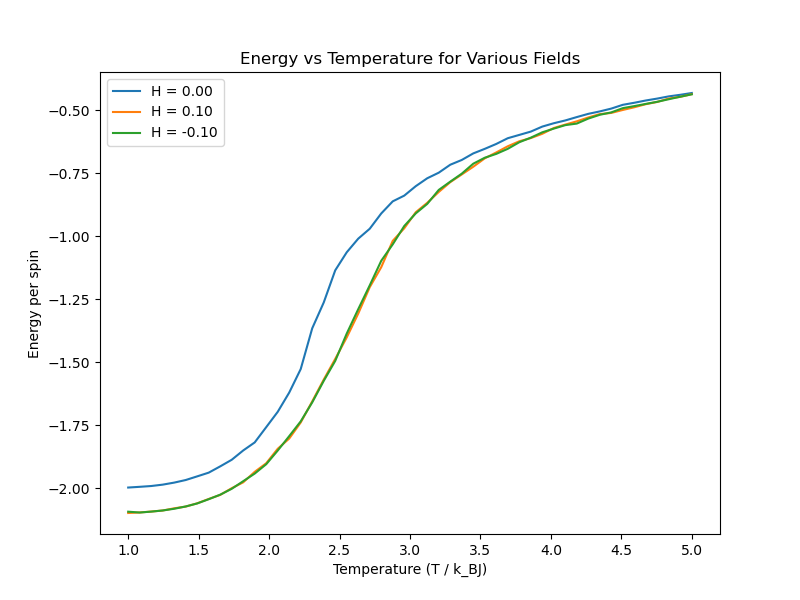
\includegraphics[width=0.8\textwidth]{Figs_Salar/heating_E-T.png}
\caption{Energy per spin as a function of temperature (\(T / k_B\)) for external fields \(H = 0.0\), \(H = 0.1\), and \(H = -0.1\). The higher energy for \(H = 0.0\) reflects the lack of a stabilizing magnetic field, while the curves for \(H = \pm 0.1\) demonstrate the influence of the external field in stabilizing spin alignments.}
\label{fig:energy_vs_temp}
\end{figure}

\subsubsection*{Magnetization and Temperature Behavior}
Figure \ref{fig:magnetization_vs_temp} shows the magnetization per spin as a function of temperature for the same external field values. For \(H = 0.0\), the magnetization drops sharply near the critical temperature, going from \(M = \pm 1.0\) in the ordered phase to \(M = 0.0\) in the disordered phase. This sharp transition is a hallmark of the 2D Ising model's phase transition.

For \(H = 0.1\), the magnetization remains positive across all temperatures, as the external field aligns spins with the field direction, suppressing the critical transition. Similarly, for \(H = -0.1\), the magnetization is negative at all temperatures due to alignment in the opposite direction. At high temperatures (\(T / k_B > 4.0\)), the magnetization approaches \(M = 0.0\) for all fields, as thermal noise dominates spin interactions.

The analytical curve for \(H = 0.0\) (dashed line) matches the simulated results well at high temperatures but shows slight discrepancies in the critical region (\(T / k_B = 2.0\) to \(T / k_B = 3.0\)). These discrepancies arise from finite lattice effects and statistical noise, as the \(20 \times 20\) lattice cannot fully capture the long-range correlations present near the critical temperature. Despite these minor deviations, the overall agreement validates the robustness of the simulation.

\begin{figure}[h!]
\centering
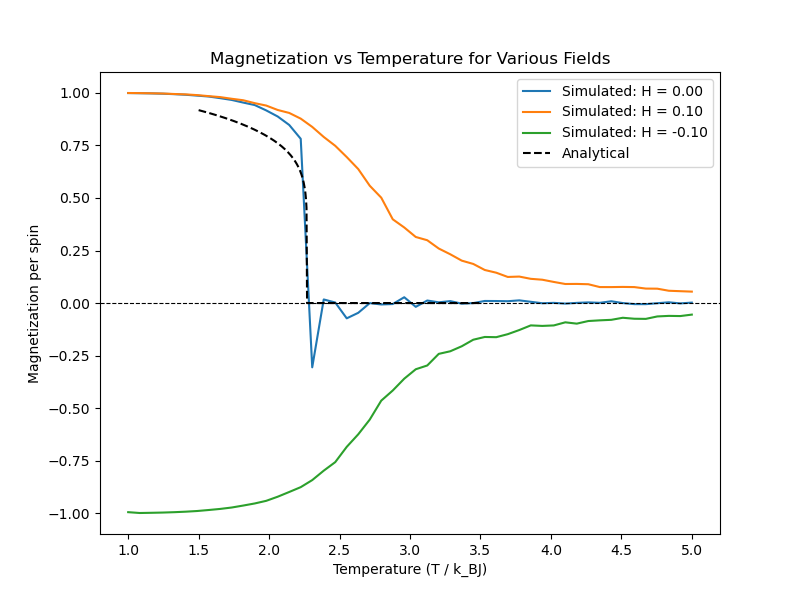
\includegraphics[width=0.8\textwidth]{Figs_Salar/heating_M-T_comparison.png}
\caption{Magnetization per spin as a function of temperature (\(T / k_B\)) for external fields \(H = 0.0\), \(H = 0.1\), and \(H = -0.1\). The dashed line represents the analytical solution for \(H = 0.0\), showing close agreement with simulated data except for small discrepancies in the critical region.}
\label{fig:magnetization_vs_temp}
\end{figure}

\subsubsection*{Effect of External Field \(H\)}
The external field \(H\) plays a significant role in stabilizing spin configurations. For \(H = 0.1\), the field aligns spins in the positive direction, leading to positive magnetization and slightly lower energy. For \(H = -0.1\), spins align in the negative direction, producing negative magnetization. The presence of the field suppresses the phase transition, maintaining a nonzero magnetization even above the critical temperature. This breaks the symmetry of the system, illustrating how small external fields can significantly influence the Ising model's behavior.

\subsubsection*{Simulation Implementation and Optimization Analysis}
The simulation code is designed to balance efficiency and accuracy, achieving high-resolution results even with a \(20 \times 20\) lattice. Each simulation run, corresponding to a single external field value (\(H = 0.0\), \(H = 0.1\), or \(H = -0.1\)), takes approximately 700 seconds to complete. This runtime corresponds to \(10^6\) iterations per temperature step, each 1 degee includes 50 temperature points. The primary computational effort lies in updating the lattice configuration, with each Metropolis step having a complexity of \(O(20 \times 20)\).

The extensive averaging over configurations ensures high-resolution energy and magnetization data, effectively compensating for the small lattice size. While the lattice size introduces finite-size effects, the code's design minimizes these effects, allowing it to capture key features such as the critical transition and field-induced behavior.

\paragraph{Alternative Implementation for Improved Efficiency}
An alternative version of the code uses an optimized approach with \(O(20 \times 20)\) complexity per iteration but converges in 500 times fewer iterations. Instead of selecting a single spin per step, this version evaluates all \(20 \times 20\) lattice points simultaneously for 500 random configurations in each Monte Carlo step. By sampling the phase space more comprehensively, it ensures faster convergence while maintaining accuracy. This version reduces the runtime to approximately 1/500th of the original code's runtime, making it ideal for larger lattices or extensive parameter studies.

\subsubsection{cooling of the lattice}

\noindent The cooling simulation code, available at uses a \(20 \times 20\) lattice with a Metropolis algorithm to study the 2D Ising model under different external magnetic fields during a cooling process. Unlike the heating simulation, this process starts at a high temperature (\(T / k_B = 10.0\)) and gradually cools down to a low temperature (\(T / k_B = 0.1\)) over 100 steps. Below, we analyze the energy and magnetization trends during cooling, compare them to the heating process, and discuss the observed phenomena.

\subsubsection*{Energy and Cooling Behavior}
Figure \ref{fig:cooling_E-T} presents the energy per spin as a function of temperature during cooling for \(H = 0.0\), \(H = 0.1\), and \(H = -0.1\). At high temperatures (\(T / k_B > 5.0\)), the energy fluctuates significantly due to the random spin alignments in the disordered phase. As the temperature decreases, the energy stabilizes and transitions to lower values. Below the critical temperature (\(T_c \approx 2.269\)), the energy rapidly decreases, reflecting the formation of ordered spin domains.

At the lowest temperatures, the energy reaches a nearly constant value, corresponding to a highly ordered state. The energy curve for \(H = 0.0\) lies slightly above those for \(H = \pm 0.1\), as the absence of an external field allows for more random spin arrangements. The curves for \(H = \pm 0.1\) show the stabilizing effect of the external field, aligning spins and reducing energy further.

Compared to the heating process, the cooling curves display more noise, especially at intermediate temperatures (\(T / k_B = 3.0\) to \(T / k_B = 5.0\)). This increased noise arises from the random initialization of the lattice and the gradual cooling process, which can trap the system in local energy minima.

\begin{figure}[h!]
\centering
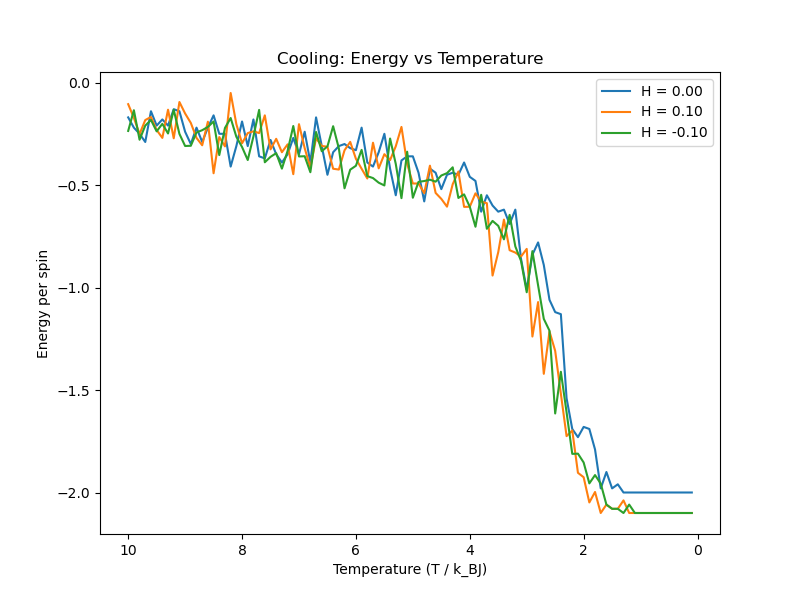
\includegraphics[width=0.8\textwidth]{Figs_Salar/cooling E-T (S).png}
\caption{Energy per spin as a function of temperature (\(T / k_B\)) during cooling for external fields \(H = 0.0\), \(H = 0.1\), and \(H = -0.1\). The energy curves exhibit more noise compared to the heating process, particularly at intermediate temperatures.}
\label{fig:cooling_E-T}
\end{figure}

\subsubsection*{Magnetization and Fluctuations During Cooling}
Figure \ref{fig:cooling_M-T} shows the magnetization per spin during cooling. For \(H = 0.0\), the magnetization fluctuates randomly between positive and negative values, particularly at low temperatures. This behavior occurs because, in the absence of an external field, the system has no preference for spin alignment direction. As the temperature approaches zero, the magnetization tends to stabilize in either the positive or negative direction, depending on the specific realization of the lattice.

For \(H = 0.1\), the magnetization is consistently positive, reflecting the field's influence in aligning spins. Similarly, for \(H = -0.1\), the magnetization remains negative. These results agree with the heating simulation, where the external field suppresses fluctuations and imposes a preferred spin alignment.

The cooling curves exhibit greater noise compared to the heating results, especially in the disordered phase (\(T / k_B > 5.0\)). This is due to the randomized initialization of spins and the limited averaging at each temperature step. The small lattice size (\(20 \times 20\)) amplifies these fluctuations, as fewer spins contribute to the magnetization calculation.

\begin{figure}[h!]
\centering
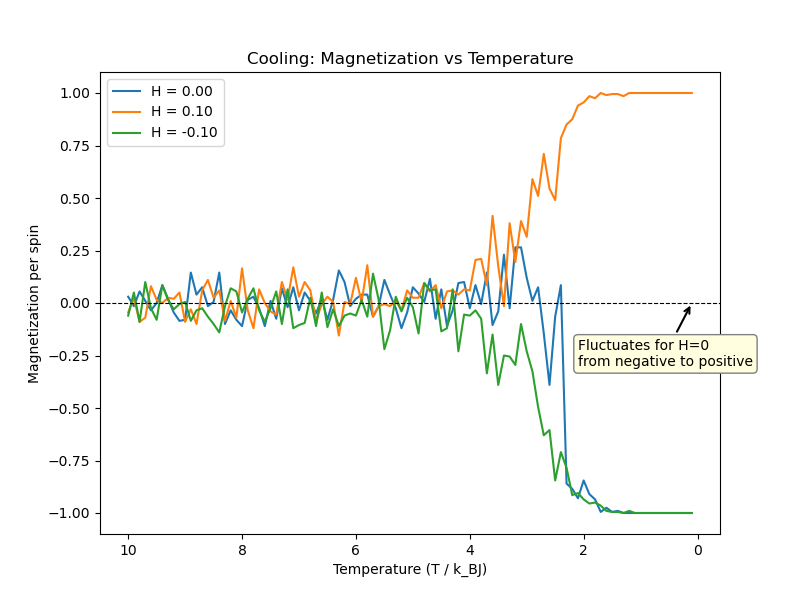
\includegraphics[width=0.8\textwidth]{Figs_Salar/cooling M-T (S).png}
\caption{Magnetization per spin as a function of temperature (\(T / k_B\)) during cooling for external fields \(H = 0.0\), \(H = 0.1\), and \(H = -0.1\). The random fluctuations for \(H = 0.0\) at low temperatures reflect the system's lack of directional preference without an external field.}
\label{fig:cooling_M-T}
\end{figure}

\subsubsection*{Comparison with Heating Results and Analytical Agreement}
The cooling results qualitatively agree with the heating process, showing similar trends in energy and magnetization. However, the cooling curves exhibit greater noise and variability due to the different initialization conditions and cooling dynamics. The increased noise is particularly noticeable in the magnetization for \(H = 0.0\), where fluctuations persist at low temperatures. These fluctuations are absent during heating, as the system begins in an ordered state.

Both the heating and cooling results align well with analytical predictions at high temperatures (\(T / k_B > 5.0\)), where the system becomes disordered. At lower temperatures, small discrepancies arise due to finite-size effects and noise in the simulation. Despite these limitations, the overall trends confirm the validity of the Metropolis algorithm and the robustness of the simulation setup.

\subsubsection*{Interpretation of Increased Noise During Cooling}
The higher noise levels during cooling stem from the randomized initialization of the lattice, where spins are initially uncorrelated.. As the system cools, it can become trapped in metastable states, leading to variability in the energy and magnetization. Additionally, the small lattice size amplifies these effects, as fewer spins contribute to the macroscopic averages.Also here i use 100000 iteration per temperature slot.

\subsubsection*{Simulation Efficiency and Performance}
The cooling simulation runs for approximately 100,000 iterations per temperature step over 100 temperature points, taking a total runtime of around 1000 seconds per external field. The modular design and efficient Metropolis updates ensure high-resolution results despite the limited lattice size. The code's flexibility allows for easy adaptation to larger lattices or alternative cooling protocols, making it a powerful tool for studying the Ising model and related systems.

\subsubsection{Sinusoidal outside field(bonus)}

 This result examines the behavior of the 2D Ising model under a sinusoidal external magnetic field, where the field oscillates as a function of time. The implementation and results focus on how varying the field's period affects energy and magnetization during heating.

\subsubsection*{Implementation of Sinusoidal Field}
The sinusoidal external magnetic field was implemented using the following time-dependent equation:
\begin{equation}
H(t) = H_0 \sin\left(\frac{2 \pi t}{\text{Period}}\right),
\end{equation}
where \(H_0 = 0.1\) is the field amplitude and "Period" determines the oscillation duration. For each time step, the field value is updated based on the current time and the selected period. This approach introduces dynamic fluctuations in the external field, contrasting with the constant fields used in the earlier heating and cooling simulations.

The simulation was performed for three field periods: \(50\), \(100\), and \(200\), using a \(20 \times 20\) lattice. The Metropolis algorithm was employed, where each spin's update considered the local interaction energy and the time-dependent external field. The results are averaged over \(100,000\) time steps for each of \(50\) temperature points in the range \(T / k_B = 1.0\) to \(T / k_B = 5.0\).

\subsubsection*{Energy vs. Temperature for Different Field Periods}
Figure \ref{fig:sinh_energy} shows the energy per spin as a function of temperature for the three field periods. At low temperatures (\(T / k_B < 2.0\)), the energy is nearly constant and close to the minimum value, as spins align to minimize both the interaction and the external field's energy. As the temperature increases, thermal fluctuations disrupt spin alignment, causing the energy to rise.

Interestingly, the energy curves for the different field periods overlap significantly, indicating that the period of the external field has a minor impact on the energy dynamics at high temperatures. However, small deviations are observed at intermediate temperatures (\(T / k_B = 2.0\) to \(T / k_B = 4.0\)), where the oscillatory nature of the field introduces subtle variations in spin alignment and energy. These differences are more pronounced for shorter field periods (\(50\)), as the rapid oscillations prevent the system from fully adapting to the field.

\begin{figure}[h!]
\centering
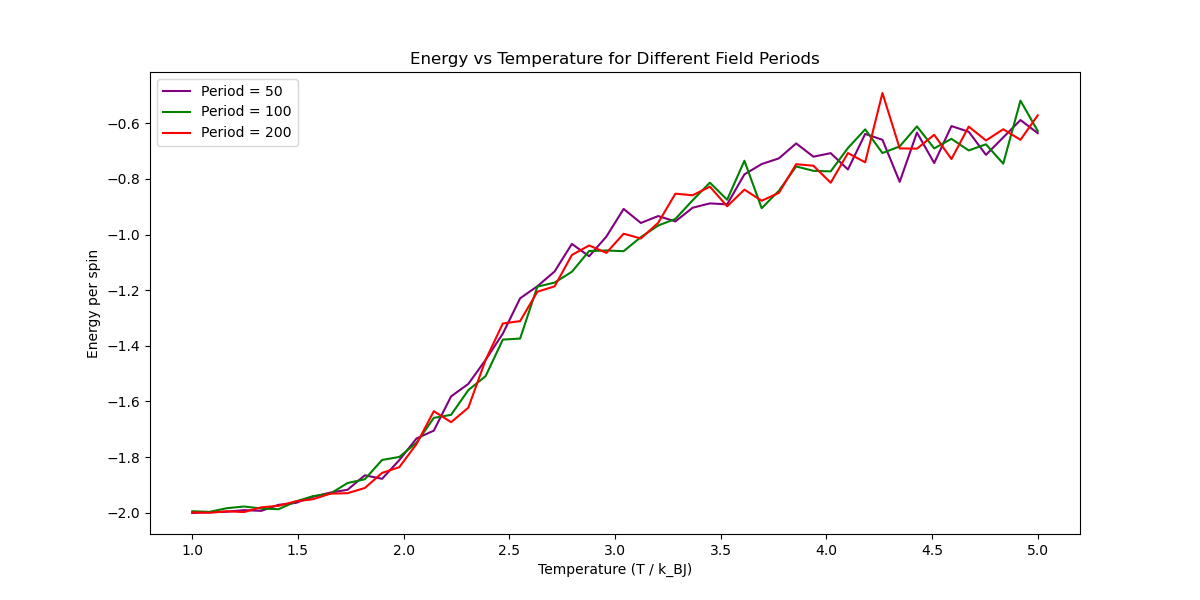
\includegraphics[width=0.8\textwidth]{Figs_Salar/SinH E-T (S).png}
\caption{Energy per spin as a function of temperature (\(T / k_B\)) for sinusoidal fields with periods of \(50\), \(100\), and \(200\). The curves are similar, with minor variations at intermediate temperatures due to differences in field oscillation rates.}
\label{fig:sinh_energy}
\end{figure}

\subsubsection*{Effect of Field Period on Energy Dynamics}
The field period affects the system's ability to adapt to the oscillating field. For shorter periods (\(50\)), the field changes more rapidly than the spin configuration can respond, leading to a more disordered state and slightly higher energy at intermediate temperatures. In contrast, for longer periods (\(200\)), the field changes more slowly, allowing the system to adapt more fully, resulting in marginally lower energy. However, these differences are small compared to the overall thermal fluctuations, which dominate at high temperatures.

\subsubsection*{Comparison with Analytical Expectations and Previous Results}
The sinusoidal field results are consistent with analytical expectations for the Ising model under dynamic fields. The energy trends at high temperatures align with those observed in the constant-field simulations, where thermal fluctuations dominate over external field effects. The results also qualitatively agree with the heating simulations in the absence of a dynamic field, with energy stabilizing at high temperatures and rising sharply near the critical temperature.

The primary distinction is the noise introduced by the oscillatory field, particularly for shorter periods. These fluctuations reflect the system's inability to fully equilibrate with the rapidly changing field, highlighting the importance of field dynamics in determining spin behavior.






\subsection{Xinyu's Results}

\subsubsection{Code in github}

All of my written code is available at: \url{https://github.com/rising1227/phys-ga2000/tree/main/2DIsingModel1}

\subsubsection{physical and coding setup}

\begin{itemize}
    \item The physical system is represented by a $m*m$ numpy array. Each spin is represented by a int8 type variable. This is the most compact variable to represent a spin. We use +1 to represent spin up$\uparrow$ and -1 to represent spin down$\downarrow$. We denote our matrice as S. We also use a function “IsingGenerationint” inside initialize.py to generate a initial spin array $S_0$
    \item A external magnetic field is denoted by a $M*M$ numpy array $B'$. $B[i][j]$ represent the external magnetic field at each point. The total energy of initial system can be calculated.
    \item A energy calculation function "CalculateEnergyint" inside initialize.py take $S$ and $B'$ as input and calculate the total energy.
    \item A transfer function “transferfunctionint” in Metropolis.py represent one step in the markov chain in the Metropolis method. It takes $S$, $B$, Total magnetization $M$, total energy $E$ and temperature $T$ as the input. It changes the $S$ internally, while outputing a renewed $M$ and $E$.
    \item Then we define a Metropolis function "metropolis" inside Metropolis.py which utilize transferfunctionint function iteratively. Also inputting the temperature $T$, $S$, $B$, $M$, $E$. This metropolis function reiterates the transfer function for many times and detect whether our system goes to thermal equilibrium. After thermal equilibrium, it outputs a averaged total energy and magnetization at a certain temperature.
    \item At main script main.py, we utilize this metropolis function many times for different temperature and external magnetic field. Finally, we can have a full curve of $E$ and $M$ as a function of temperature for different external field.
\end{itemize}

\subsubsection{Selecting reasonable system size and number of metropolis steps}

Theoretically, a discontinuous phase transition is only happening in a infinitely large physical system(particle number $N \rightarrow +\infty$). So we'd probably like to simulate a system as large as possible. Other than that, for a system in thermal equilibrium, we have the fluctuation-dissipation theorem

\begin{equation}
    \Delta E^2 = k_B T^2 C_V
\end{equation}

Since both Energy and $C_V$ scales proportionally with N, we know that the fluctuation for relative energy scales as:

\begin{equation}
    \frac{\Delta E}{E} \propto \frac{1}{\sqrt{N}} = \frac{1}{m}
\end{equation}

We can actually easily test this relation by calculating the energy variance w.r.t. system size and the simulation result goes as follows\ref{fluctuation}. In this figure, we chose very large metropolis steps(50 million) and relatively small system to ensure thermal equilibrium(we use the parameter T'=3 here):

\begin{figure}[H]
    \centering
    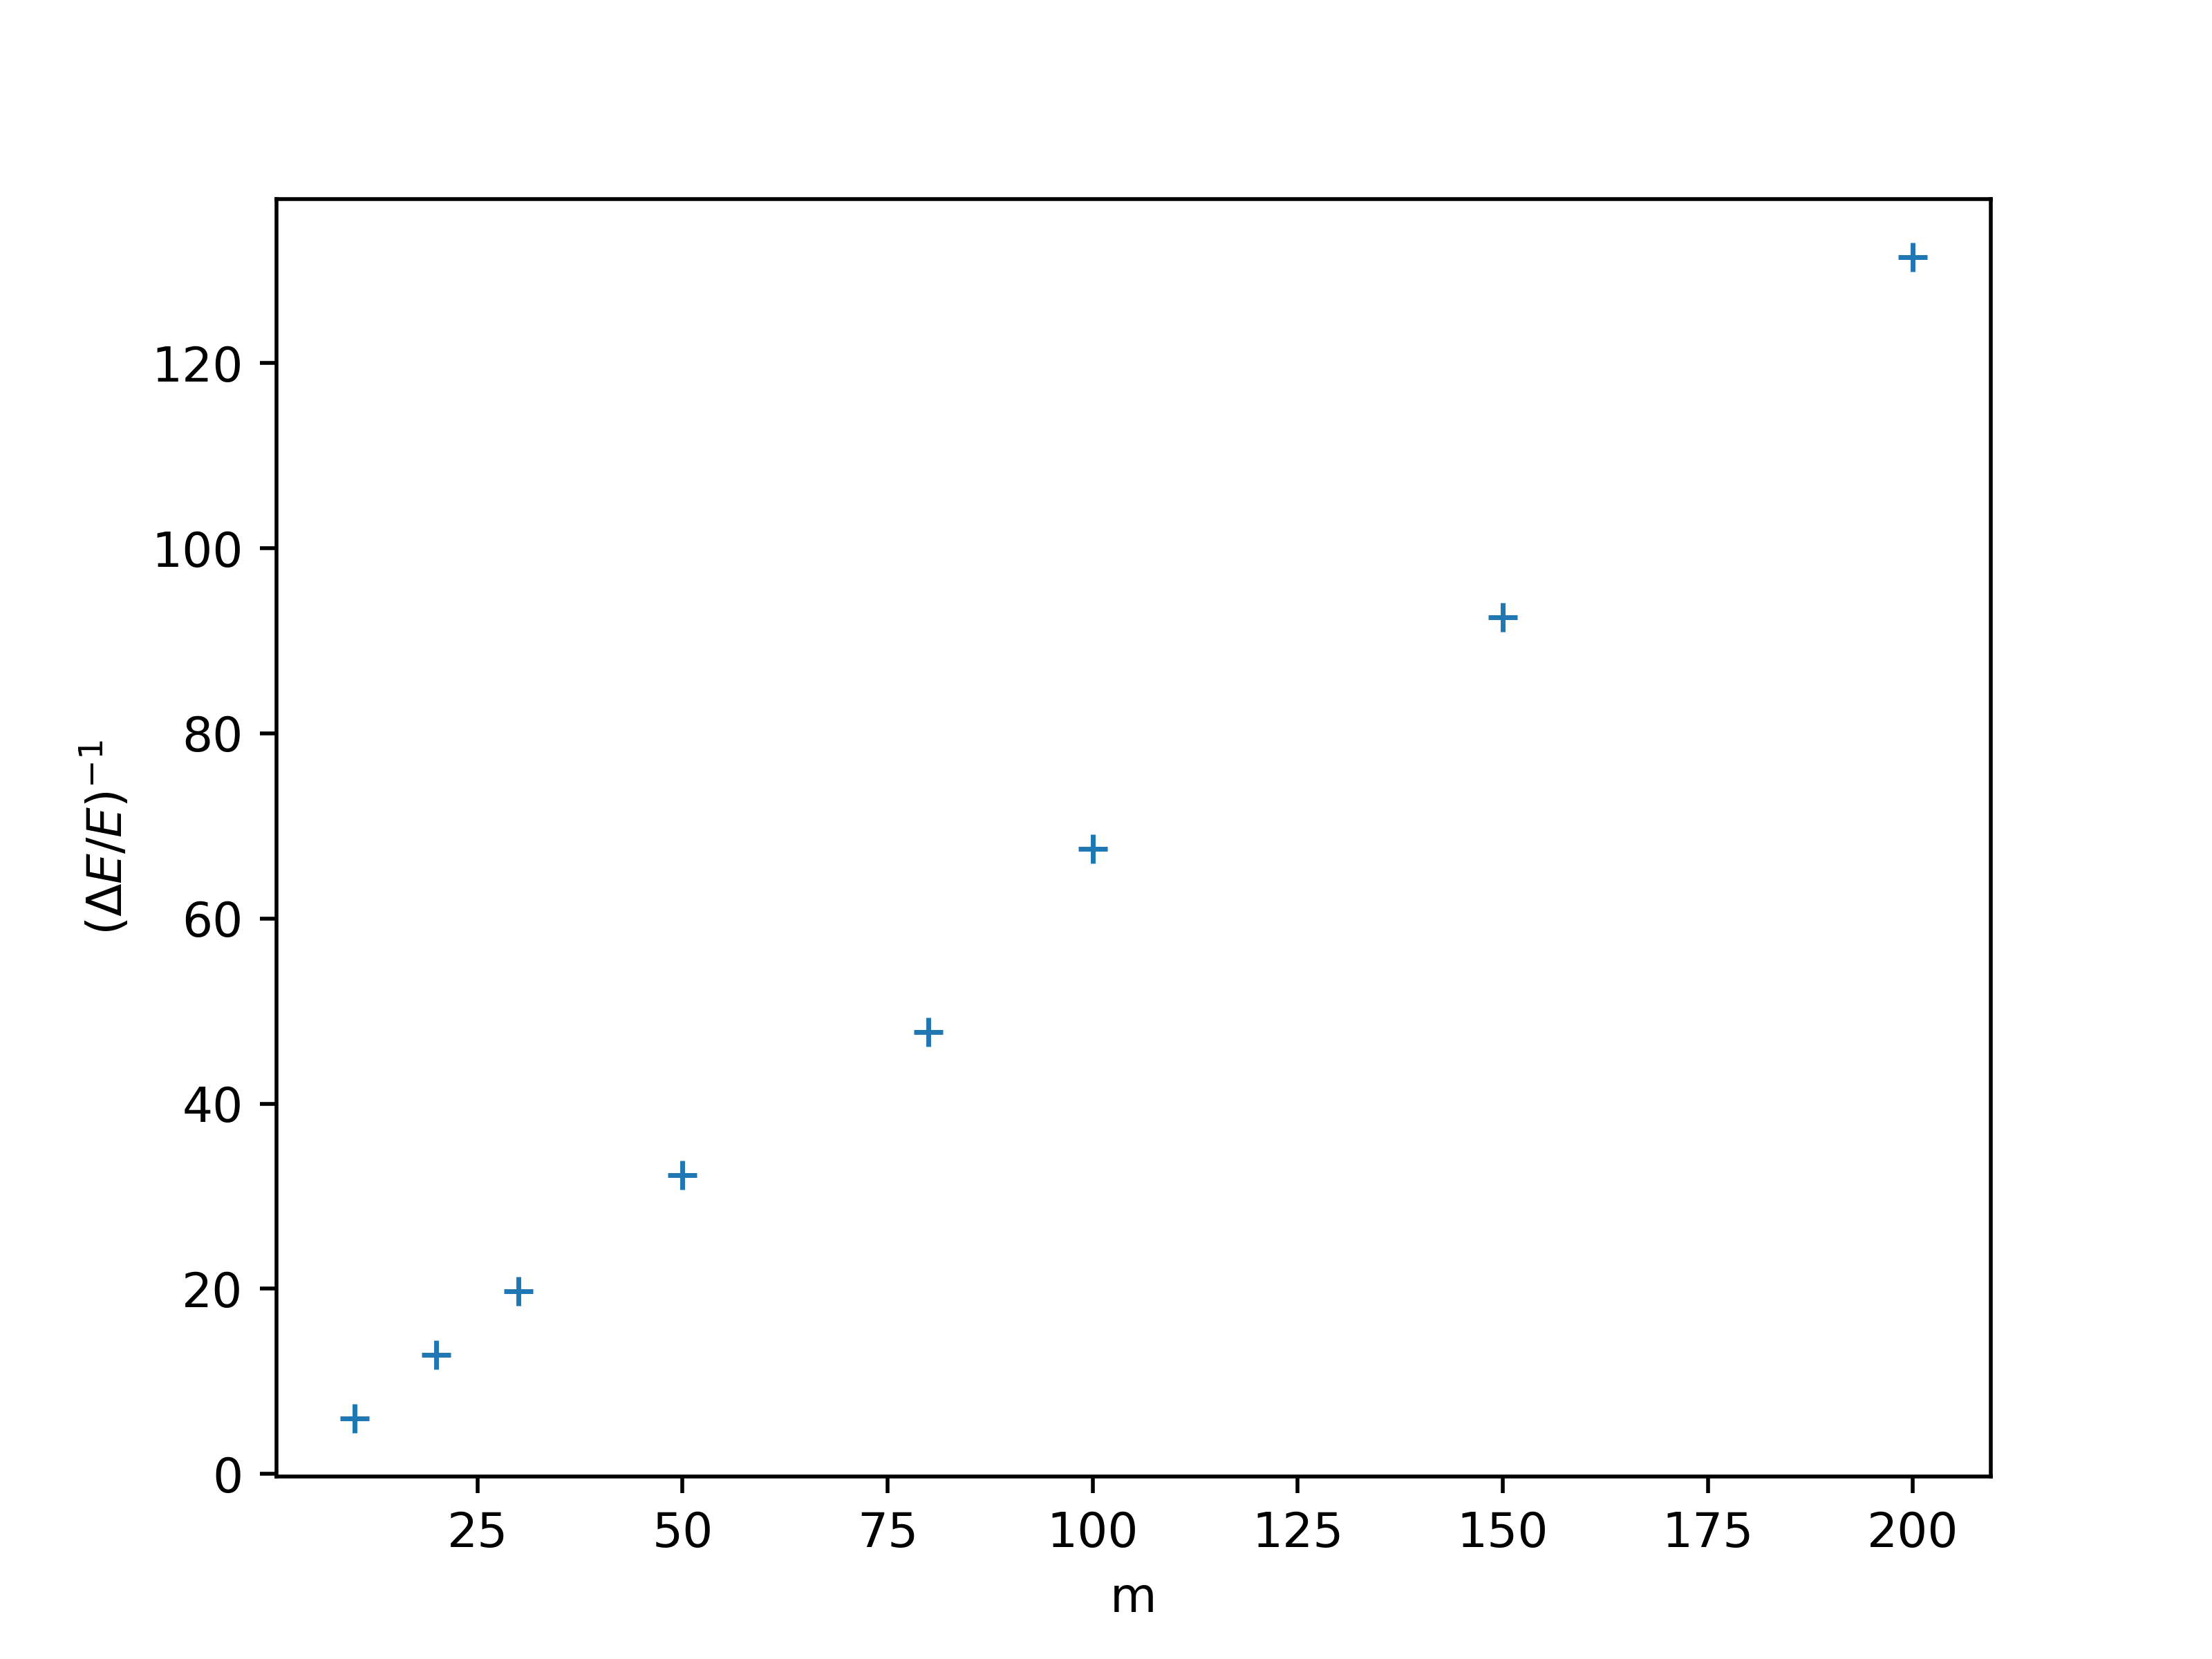
\includegraphics[scale = 0.7]{Figs_XYL/fluctuation-ensemblesize.png}
    \caption{relationship between energy fluctuation and the size of ensemble(m)}
    \label{fluctuation}
\end{figure}

We can see that the calculation result fits quite well with fluctuation-dissipation theorem.(i.e. the relative fluctuation $\Delta E/E$ is proportional to $m^{-1}$). To be more exact, we have:

\begin{equation}
    \Delta E/E = \frac{1}{0.6016 * m}
\end{equation}

% \textbf{This is not only pedagogical as a test of textbook theorem but will also be more than useful as a determination on whether a system has realized thermal equilibrium}. We actually fitted a function for expectation energy fluctuation against the system size. In a real metropolis process, when the energy fluctuation of an ensemble goes close to our theoretical value, we believe that the thermal equilibrium is reached and the calculated average energy is credible.



This shows that the larger the system is, the less fluctuation we can get and thus it's easier for us to do simulation and get the theoretical energy expectation for a certain temperature in a limited ensemble of states.

Also, for larger system, it takes longer times to reach thermal equilibrium if the contact rate is fixed. In a Markov chain, by modifying physical system each time by flipping one spin and setting up a temperature-determined acceptance rate. The number of steps required to reach equilibrium is at least proportional to the size of system $m^2$(since there are $O(m^2)$ amount of spins need to be flipped when temperature changed). Simulating large system significantly enlarge the computational resources. So there's a trade-off on selecting the size of spin system. In my work, I made significant effort on optimize the code to make it run faster.

\subsubsection{Optimization on code}

Several method is implimented to speed up the code. Here's something I've done or will do in short time:

\begin{itemize}
    \item I've utilize the int8 variable type which is the smallest int type to represent a spin(I've tried to write a code with bool type, but I find that it's not faster since the type transfer function is slow)
    \item I've also implimenting the "multiprocessing" module in python in order to run different part of the program parallel. This significantly improve the calculation speed in 10 times(since my mac only have 10 cores).
    \item The slowest step in our code is actually the for loop inside python when doing metropolis steps. I'm thinking about using C++ to work faster in loops. Another possible way is that, for a large system, when you randomly chose two point, for most of the case they are not in contact with each other. So that you can actually do more than one attempt of spin flipping inside a cycle of loop. I'll try to see whether this work later.
\end{itemize}
 

\subsubsection{Result and discussion}

After taking enough effort on getting equilibrium and optimization. I'm able to run a 1000*1000 spin system and having 400 data points between $T' = 0$ and $T' = 5$. The $E'-T'$ curve goes as follows:

\begin{figure}[H]
    \centering
    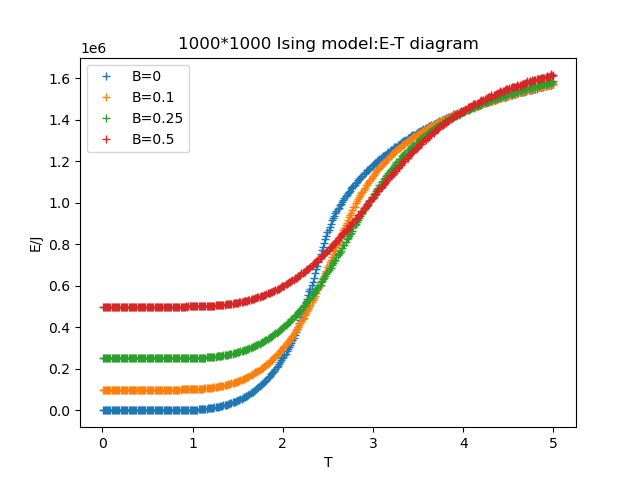
\includegraphics[scale = 0.7]{Figs_XYL/E-T_withB_diagram(latest).png}
    \caption{relationship between energy and temperature for different external field}
    \label{ETXinyu}
\end{figure}

Here, since the system have a discrete $Z_2$ global symmetry, we only plotted the energy temperature curve with positive magnetization. Here I also do the renormalization of energy such that at the ground state of this system at zero external field has zero energy.

We also plotted the magnetization of the system w.r.t. temperature and external magnetization.

\begin{figure}[H]
    \centering
    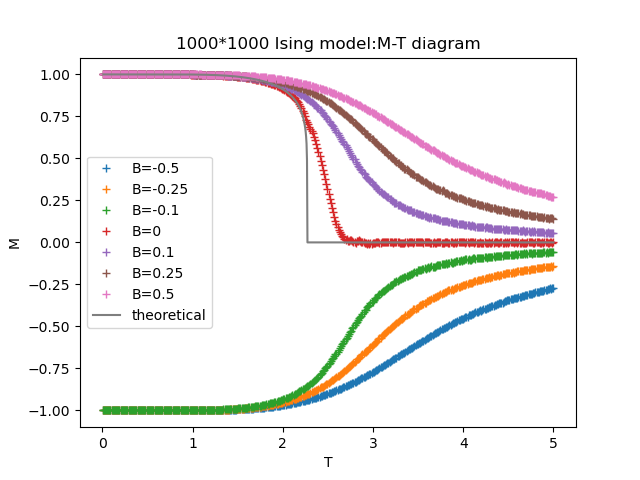
\includegraphics[scale = 0.7]{Figs_XYL/M-T_withB_diagram(latest).png}
    \caption{relationship between magnetization and temperature for different external field}
    \label{ETXinyu}
\end{figure}

From this figure we can see the discrete symmetry more clearly. We can see that the lower the external field the closer it's to the theoretical magnetization value. However, a perfect theoretical function between M and T is only for a infinitely large system and is thus not available in our simulation.

The cooling part result will be shown in our final paper.

\subsection{Tongzhou's Results}
My code is available at: \url{https://github.com/rising1227/2DIsingModel.git}.

In my simulations the system size is $50 \times 50$ spins. For large systems, it is expected that the Markov chain needs more steps to converge as there are more possible configurations. Small systems are relatively unstable in the sense that they are more likely to shift between a mainly spin up configuration and a mainly spin down configuration at finite temperatures below the critical temperature. Newmann uses $20 \times 20$ spins in his textbook problem \cite{newman2013computational}.

Figure \ref{fig:energy} shows the energy $E^\prime$ as a function of temperature $T^\prime$ for various values of magnetic field $H^\prime$. The system size is $50 \times 50$ spins. The system is initially at $T^\prime = 0$ with all spins aligned $s=1$ and is then heated up.

The $E^\prime$-$T^\prime$ curves for negative $H^\prime$ starts to coincide with those for positive $H^\prime$ at certain temperatures. This indicates that the spins flipped to align with the magnetic field to minimize the energy. The coincidence happens at lower temperatures for larger magnitudes of $H^\prime$. This is because under our choices of $H^\prime < 8$, when the spins in the system are mainly pointing up, flipping a spin to point down increases the energy and is unfavorable. For larger magnitudes of $H^\prime$, the increase in energy is smaller and the flip is more likely to happen.
\begin{figure}[H]
    \centering
    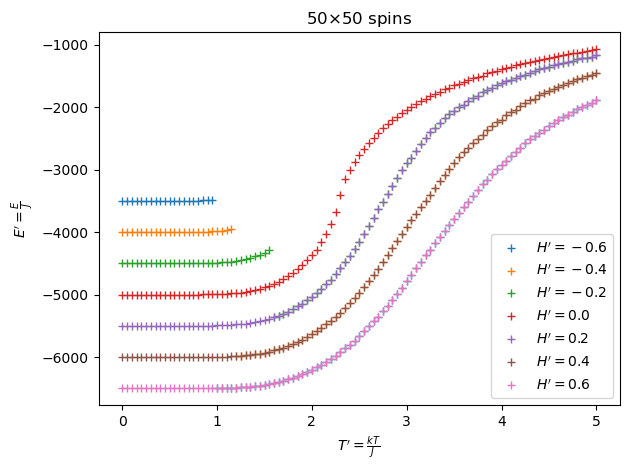
\includegraphics[scale = 0.7]{Figs_TW/energy_N50.png}
    \caption{Energy $E^\prime$ as a function of temperature $T^\prime$ for various values of magnetic field $H^\prime$. The system size is $50 \times 50$ spins. The system is initially at $T^\prime = 0$ with all spins aligned $s=1$ and is then heated up.}
    \label{fig:energy}
\end{figure}

Figure \ref{fig:magnetization} shows the magnetization $M$ as a function of temperature $T^\prime$ for various values of magnetic field $H^\prime$. The system size is $50 \times 50$ spins. The system is initially at $T^\prime = 0$ with all spins aligned $s=1$ and is then heated up.

For the case of $H^\prime = 0$, the data fluctuate about the analytical value 0 around the critical temperature $T^\prime_c = 2.269185$. We observe that around the critical temperature, the magnetization of the states in the Markov chain does not converge but constantly shifts between $\pm 1$. For the data of the $H^\prime = 0$ curves in Figures \ref{fig:energy} and \ref{fig:magnetization}, $5 \times 10^5$ Markov chain steps were taken for $0 \leq T_c^\prime < 2.1$, $5 \times 10^7$ steps were taken for $2.1 \leq T_c^\prime \leq 2.5$, and $1 \times 10^7$ steps were taken for $2.5 < T_c^\prime \leq 5$. The computation takes about two hours to run. We expect that increasing the steps taken around the critical temperature and averaging over more steps will give results closer to the analytical behavior.

The $M$-$T^\prime$ curves for negative $H^\prime$ flip to become symmetric with those for positive $H^\prime$ at certain temperatures. The flip happens at lower temperatures for larger magnitudes of $H^\prime$. This agrees with the behavior of the $E^\prime$-$T^\prime$ curves.
\begin{figure}[H]
    \centering
    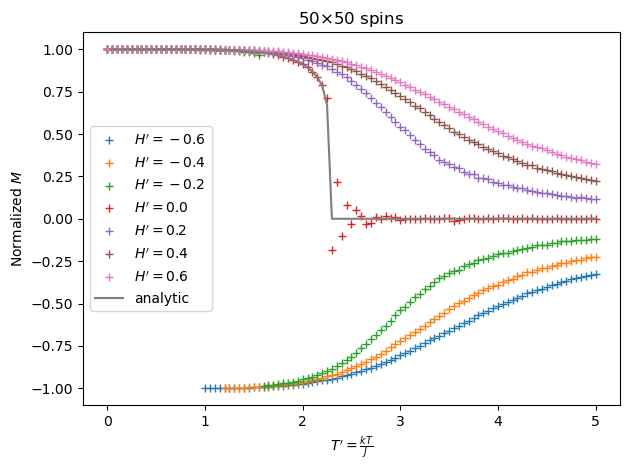
\includegraphics[scale = 0.7]{Figs_TW/magnetization_N50.png}
    \caption{Magnetization $M$ as a function of temperature $T^\prime$ for various values of magnetic field $H^\prime$. The system size is $50 \times 50$ spins. The system is initially at $T^\prime = 0$ with all spins aligned $s=1$ and is then heated up.}
    \label{fig:magnetization}
\end{figure}

Figure \ref{fig:cool_energy} shows the energy $E^\prime$ as a function of temperature $T^\prime$ for various values of magnetic field $H^\prime$. The system size is $50 \times 50$ spins. The system is initially at $T^\prime = 5$ with random spin orientations and is then cooled down.

In contrast to Figure \ref{fig:energy}, now the $E^\prime$-$T^\prime$ curves for negative $H^\prime$ coincide with those for positive $H^\prime$ everywhere. This makes sense because we are now starting with a random spin configuration and cooling down. The curve for $H^\prime = 0$ looks similar to the one in Figure \ref{fig:energy}.
\begin{figure}[H]
    \centering
    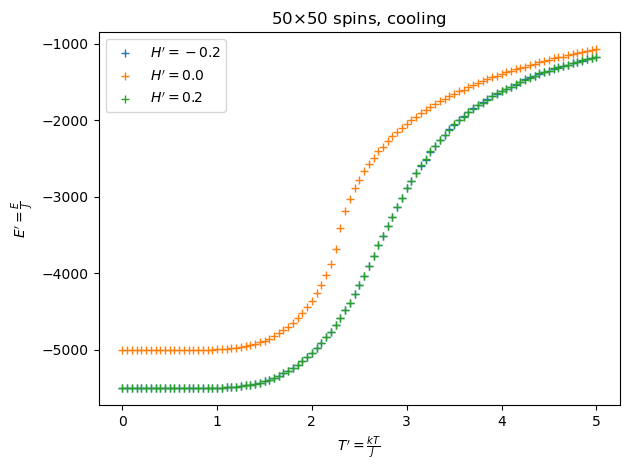
\includegraphics[scale = 0.7]{Figs_TW/cool_energy_N50.png}
    \caption{Energy $E^\prime$ as a function of temperature $T^\prime$ for various values of magnetic field $H^\prime$. The system size is $50 \times 50$ spins. The system is initially at $T^\prime = 5$ with random spin orientations and is then cooled down.}
    \label{fig:cool_energy}
\end{figure}

Figure \ref{fig:cool_magnetization} shows the magnetization $M$ as a function of temperature $T^\prime$ for various values of magnetic field $H^\prime$. The system size is $50 \times 50$ spins. The system is initially at $T^\prime = 5$ with random spin orientations and is then cooled down.

In contrast to Figure \ref{fig:magnetization}, now the $M$-$T^\prime$ curves for negative $H^\prime$ are symmetric to those for positive $H^\prime$ everywhere. This makes sense because we are now starting with a random spin configuration and cooling down. The curve for $H^\prime = 0$ looks similar to the one in Figure \ref{fig:magnetization}.

\begin{figure}[H]
    \centering
    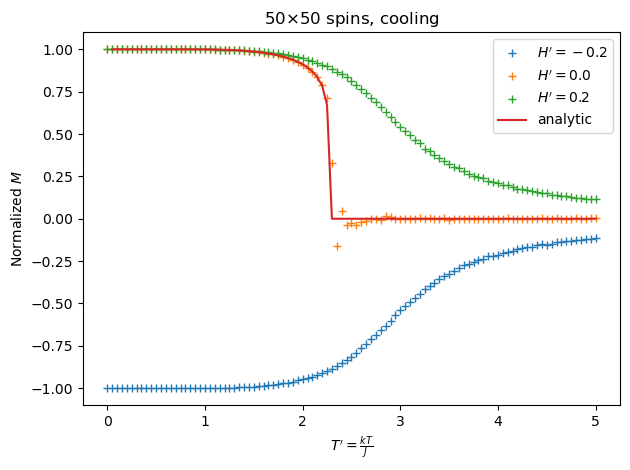
\includegraphics[scale = 0.7]{Figs_TW/cool_magnetization_N50.png}
    \caption{Magnetization $M$ as a function of temperature $T^\prime$ for various values of magnetic field $H^\prime$. The system size is $50 \times 50$ spins. The system is initially at $T^\prime = 5$ with random spin orientations and is then cooled down.}
    \label{fig:cool_magnetization}
\end{figure}

\bibliographystyle{unsrt}
\bibliography{refs}

\end{document}
